\documentclass[12pt]{article}
\usepackage[utf8]{inputenc}
\usepackage{titling}
\newcommand{\subtitle}[1]{%
  \posttitle{%
    \par\end{center}
    \begin{center}\large#1\end{center}
    \vskip0.5em}%
}
\usepackage{graphicx}
\usepackage{tikz}
\usepackage{siunitx}
\usepackage{setspace}
\usepackage{fancyhdr}
\usepackage{gensymb}
\usepackage{amsmath}
\usepackage{amsfonts}
\usepackage{amssymb}
\usepackage{parskip}
\usepackage{float}
\usepackage{gensymb}
\usepackage{hyperref}
\usepackage{amsthm}
\usepackage [english]{babel}
\usepackage [autostyle, english = american]{csquotes}
\MakeOuterQuote{"}
\usepackage{comment}
\usepackage[letterpaper, margin=1in]{geometry}

%\pagestyle{fancy}
%\fancyhf{}
\begin{document}
\doublespacing
\title{The Use of Generating Functions in Solving Combinatorial Problems}
\date{}
\maketitle
\begin{center}
\end{center}
\newpage
\tableofcontents
\newpage

\section{Introduction}
While learning combinatorics to strengthen my math contest skills, I was fascinated by how combinatorics could solve and model real-world problems so precisely and elegantly. I learned many concepts through my textbooks and math circle meetings. I would be surprised at how easily generating functions could be used to create simple proofs for difficult problems. Due to their power in many topics such as in finding closed forms for recurrence relations, proving identities, convolutions, etc., I wished to explore them further. However, not all of these will be explored in the investigation because of the complexity of some topics.

Thus, I would like to use this investigation deepen my own understanding in generating functions through proofs involving different ways of using generating functions.

To do so, this investigation will first define generating functions and explore its properties. Then, proofs of identities using both generating functions and combinatorical arguments will be shown to demonstrate the strengths of generating functions. Finally, the investigation will explore the application of generating functions in solving a combinatorical problem involving probability.
\section{Definitions and Operations}
"A generating function is a clothesline on which we hang up a sequence of numbers for display." - Wilf, generatingfunctionology, page 1.

The definition of generating functions will not be given immediately. Instead, intuition will be given to illustrate how generating functions can be created through an example.
\subsection{Intuition}
Consider two fair six-sided dice. Suppose we roll the dice and want to find the number of ways for each possible sum of the two numbers on the two dice. This can be done with a simple table, where the first row and first column represent the individual dice numbers, and the intersection of rows and columns represent their sums. 
\begin{table}[H]
\centering
\begin{tabular}{|c|c|c|c|c|c|c|c|}
\hline
Sum of Dice & Dice 2 & 1 & 2 & 3 & 4  & 5  & 6  \\ \hline
Dice 1      &        &   &   &   &    &    &    \\ \hline
1           &        & 2 & 3 & 4 & 5  & 6  & 7  \\ \hline
2           &        & 3 & 4 & 5 & 6  & 7  & 8  \\ \hline
3           &        & 4 & 5 & 6 & 7  & 8  & 9  \\ \hline
4           &        & 5 & 6 & 7 & 8  & 9  & 10 \\ \hline
5           &        & 6 & 7 & 8 & 9  & 10 & 11 \\ \hline
6           &        & 7 & 8 & 9 & 10 & 11 & 12 \\ \hline
\end{tabular}
\caption{Sum of the numbers on the faces of dice}
\end{table}
There is one possibility for the sum to be 2, two possibilities for the sum to be 3, three possibilities for the sum to be 4, four possibilities for the sum to be 5, etc.

We wish to capture this information succinctly. We create a polynomial that tries to do so.

Consider the polynomial \[x^2 + 2x^3 + 3x^4 + 4x^5 + 5x^6 + 6x^7 + 5x^8 + 4x^9 + 3x^{10} + 2x^{11} + x^{12}.\] In the polynomial, each term encapsulates some information. The exponent of $x$ indicates which value for the sum of dice we examine, and the coefficient of $x$ indicates how many possible ways there are to roll this specific value. For example, there are two ways to have the dice sum to 3: 1 and 2 is one possibility and the other is 2 and 1. This is seen in the term $2x^3$.

The $x$ in the polynomial does not represent anything in particular and so it does not have any meaning by itself, but it can be thought of as a variable whose sole purpose is to make manipulation of expressions convenient. For this reason, plugging in specific values of $x$ into the polynomial may not always be useful, but the convenience will be seen in the following sections. 
\subsection{Definition}
More generally, we can consider the sequence $a_k$, when the sequence is defined for all non-negative integers $k$. Then, the generating function of $a_k$ is defined as
\[F(x) = a_0 x^0 + a_1 x^1 + a_2 x^2 + a_3 x^3 + \cdots = \sum_{i=0}^\infty a_i x^i.\]

In our example with the sum of two dice, the sequence $a_k$ can be defined as $a_k$ equals the number of possible ways for the sum of the two dice to equal $k$.
\subsection{Operations}
\subsubsection{Addition}
Addition and subtraction are natural operations for generating functions. Suppose we have two sequences, $a_k$ and $b_k$, where $F(x) = \sum_{i=0}^\infty a_i x^i$ and ${G(x) = \sum_{i=0}^\infty b_i x^i}$. Let $H(x)$ be the sum of the two generating functions. Then,
\[H(x) = \left(\sum_{i=0}^\infty a_i x^i \right)+ \left( \sum_{i=0}^\infty b_i x^i \right) = \sum_{i=0}^\infty (a_i x^i + b_i x^i) = \sum_{i=0}^\infty (a_i + b_i) x^i.\]
Thus, each individual term of $H(x)$ is evaluated by taking the sum of the two terms from $F(x)$ and $G(x)$ with the same $x^k$.

\begin{sloppypar}For example, suppose we have both a fair six-sided die and a fair four-sided die and we want to find the total number of ways to end up with a number on top of a face. Then, ${F(x) = x + x^2 + \cdots + x^6}$ is the generating function for the six-sided die and ${G(x)= x + x^2 + x^3 + x^4}$ is the generating function for the four-sided die, so the sum of the generating functions is ${F(x)+G(x)=2x+2x^2+2x^3+2x^4+x^5+x^6}$.
\end{sloppypar}
\subsubsection{Multiplication}
\label{multiplication}
Notice that the generating function for rolling a fair six-sided die is \[F(x) = x+x^2+x^3+x^4+x^5+x^6.\] Squaring this generating function yields \[F(x)^2 = (x+x^2+x^3+x^4+x^5+x^6)^2\]\[=x^2 + 2x^3 + 3x^4 + 4x^5 + 5x^6 + 6x^7 + 5x^8 + 4x^9 + 3x^{10} + 2x^{11} + x^{12}.\] This is the same generating function as the generating function for the number of ways for each possible sum of the two faces after rolling two six-sided dice.

This multiplication can be seen more succinctly in this table, where the polynomial in the first row is multiplied by the polynomial in the first column.
\begin{table}[H]
\centering
\begin{tabular}{|c|l|l|l|l|l|l|}
\hline
Product of Polynomials & \multicolumn{1}{c|}{$x^1$} & \multicolumn{1}{c|}{$x^2$} & \multicolumn{1}{c|}{$x^3$} & \multicolumn{1}{c|}{$x^4$} & \multicolumn{1}{c|}{$x^5$} & \multicolumn{1}{c|}{$x^6$} \\ \hline
$x^1$                  & $x^{2}$                    & $x^{3}$                    & $x^{4}$                    & $x^{5}$                    & $x^{6}$                    & $x^{7}$                    \\ \hline
$x^2$                  & $x^{3}$                    & $x^{4}$                    & $x^{5}$                    & $x^{6}$                    & $x^{7}$                    & $x^{8}$                    \\ \hline
$x^3$                  & $x^{4}$                    & $x^{5}$                    & $x^{6}$                    & $x^{7}$                    & $x^{8}$                    & $x^{9}$                    \\ \hline
$x^4$                  & $x^{5}$                    & $x^{6}$                    & $x^{7}$                    & $x^{8}$                    & $x^{9}$                    & $x^{10}$                   \\ \hline
$x^5$                  & $x^{6}$                    & $x^{7}$                    & $x^{8}$                    & $x^{9}$                    & $x^{10}$                   & $x^{11}$                   \\ \hline
$x^6$                  & $x^{7}$                    & $x^{8}$                    & $x^{9}$                    & $x^{10}$                   & $x^{11}$                   & $x^{12}$                   \\ \hline
\end{tabular}
\caption{Product of terms of polynomials}
\end{table}
Note the similarity to the first table. The numerical values in the first table are now the exponents of $x$ in this table. The act of adding together the numbers on the two dice is similar to multiplying together two powers of $x$, which adds the numerical values of the exponents. After the multiplication of each possible choice of pairs from the two polynomials, each term is added together.

This implies that multiplying generating functions is similar to choosing all possible choices of terms (or events) from both generating functions, combining them in a way by adding the exponents, counting the total number of ways to arrive at that exponent, and then adding together other possible choices of terms (or events).
\begin{sloppypar}Indeed, for two generating functions $F(x)=a_0 +a_1 x + a_2 x^2 + \cdots=\sum_{i=0}^\infty a_i x^i$ and ${G(x)=b_0 + b_1 x + b_2 x^2 + \cdots=\sum_{i=0}^\infty b_i x^i}$, the coefficient of $x^k$ of the product $F(x)G(x)$ is equal to \end{sloppypar}\[a_0 b_k + a_1 b_{k-1} + a_2 b_{k-2} + \cdots + a_k b_0 = \sum_{i=0}^k a_i b_{k-i}.\] \begin{sloppypar}This is because to contribute to the coefficient of $x^k$, the two terms being multiplied together must have exponents of $x$ that sum to $k$. These are the pairs ${(a_0 x^0, b_k x^k), (a_1 x^1, b_{k-1} x^{k-1}), \cdots, (a_k x^k, b_{0} x^{0})}$. For this reason, all of those terms and only those terms are seen in the expression above for the coefficient of $x^k$.\end{sloppypar}

Then, the product of $F(x)$ and $G(x)$ can be written as \begin{equation}\label{multiplication operation}F(x)G(x)=\sum_{i=0}^\infty a_i x^i\sum_{i=0}^\infty b_i x^i=\sum_{k=0}^\infty \left(x^k\sum_{i=0}^k a_i b_{k-i}\right),\end{equation} where the inner sum groups together all terms that have the same exponent of $x$, and the outer sum adds them all together for all exponents of $x$ (Goemans 3).

This mimics the act of adding together the faces of two dice. To have the dice sum to 7, we can have the possibility of a 1 and a 6, 2 and a 5, 3 and 4, 4 and 3, 5 and 2, or 6 and 1. In the expansion of \[(x+x^2+x^3+x^4+x^5+x^6)(x+x^2+x^3+x^4+x^5+x^6),\] this is equivalent to choosing the pairs of terms $x$ and $x^6$, $x^2$ and $x^5$, up to $x^6$ and $x$ from the first and second generating function, respectively, multiplying the values in the pairs together and then adding them together with the other pairs.

These operations themselves should demonstrate how generating functions can potentially be useful. While $x$ may not have value in itself, we notice how expanding the factored form of the generating function mirrors how we can choose two numbers from the faces of dice and add them together. For the expansion, the presence of $x$ is necessary.
\section{Applications}
Generating functions can be used to prove identities and for solving general problems. For clarity, the end of proofs will be marked with the symbol to the right. \qed 
\subsection{Identities}
Generating functions are an effective way of showing that a combinatorical identity is true for all possible conditions.
\subsubsection{Vandermonde's Identity}
We define binomial coefficients as follows for convenience. \[ \binom{a}{b}= \begin{cases} 
      \frac{a!}{b! (a-b)!} & a\ge b \\
      0 & a< b 
   \end{cases}.
\] Note that when $a\ge b$, the definition is as expected, but when $a<b$, there are no ways to pick $b$ items from $a$ total since there are not enough items. For this reason, the binomial is defined to equal 0 in that case.

We wish to prove Vandermonde's identity, which states that \[\binom{m+n}{r}=\sum_{k=0}^{r}\binom{m}{k}\binom{n}{r-k}\]
for all non-negative integers $r, m, n$.

For example, when $m=3, n=4, r=4$, the left hand side evaluates to $\binom{3+4}{4}=35$, while the right hand side evaluates to \[\sum_{k=0}^{4} \binom{3}{k}\binom{4}{4-k}=\binom{3}{0}\binom{4}{4} + \binom{3}{1}\binom{4}{3}+\binom{3}{2}\binom{4}{2}+\binom{3}{3}\binom{4}{1}+\binom{3}{4}\binom{4}{0}\]\[=1\cdot1 + 3\cdot4+3\cdot6+1\cdot4+0\cdot1=35.\]

This problem is taken from Zhao's "Lecture 10 : A Contest of Contests" on page 3.
\begin{proof}
The expression $\binom{m+n}{r}$ is difficult to manipulate. The binomial expansion \begin{equation}\label{binomial expansion}(1+x)^a = \sum_{r=0}^a \binom{a}{r} x^r\end{equation} inspires the following step, since we notice that the value of the exponent is the same as the top of the binomial. First, notice that we can increase the upper bound of the summation, since when $r>a, \binom{a}{r}=0$. Then, $(1+x)^a = \sum_{r=0}^\infty \binom{a}{r} x^r$. We consider the generating function \[(1+x)^{m+n}=\sum_{r=0}^\infty \binom{m+n}{r}x^r.\]
Inspired by how the right hand side of the identity we wish to prove has binomials with $m$ and $n$ in the top of the binomial, we manipulate the generating function as follows.
\[(1+x)^{m+n}=(1+x)^m (1+x)^n = \left(\sum_{k=0}^\infty \binom{m}{k} x^k\right)\left(\sum_{k=0}^\infty \binom{n}{k} x^k\right).\] Notice that equation \ref{binomial expansion} is used to expand both $(1+x)^m$ and $(1+x)^n$. Then, using the property of multiplication of equation \ref{multiplication operation} in section \ref{multiplication} by treating each each of the infinite sums as a generating function,
\[\left(\sum_{k=0}^\infty \binom{m}{k} x^k\right)\left(\sum_{k=0}^\infty \binom{n}{k} x^k\right) = \sum_{r=0}^\infty x^r\left(\sum_{k=0}^r \binom{m}{k}\binom{m}{r-k}\right).\]
Then, since \[\sum_{r=0}^\infty \binom{m+n}{r}x^r = (1+x)^{m+n} = \sum_{r=0}^\infty x^r\left(\sum_{k=0}^r \binom{m}{k}\binom{m}{r-k}\right)\] is an identity that is true for all $x$ (because the generating functions can be truncated to a finite polynomial when $r>m+n$), comparing coefficients of $x^r$ yields \[\binom{m+n}{r} = \sum_{k=0}^r \binom{m}{k}\binom{m}{r-k},\] which proves the identity. 
\end{proof}

Generating functions are not the only way to prove this identity, as this can also be done with a committee-making argument.
\begin{proof} Suppose we wish to make an $r$-person committee from a group of $m+n$ total people. We number the people from $1$ to $m+n$ and then split the people into two groups: the people numbered $1$ through $m$ in the first group and the remaining $n$ people in the second group. Then, there are up to $r$ ways to determine the number of people to choose from each of the two groups. We can choose none from the first group and $r$ from the second group, or one from the first group and $r-1$ from the second, etc. If we choose $k\le r$ people from the first group, we must choose $r-k$ from the second in order to create the desired group size. For each possible value of $k$, there is $\binom{m}{k}$ ways to choose the $k$ from the first group and $\binom{n}{r-k}$ from the second group. Since these choices are independent, the number of possibilities are multiplied together and then added for all possible choices of $k$. This proves the identity \[\binom{m+n}{r} = \sum_{k=0}^r \binom{m}{k}\binom{m}{r-k}.\] \end{proof}

The presence of several proofs of this identity does not detract from the usefulness of generating functions. Instead, it demonstrates how the generating functions can model real-world choices in abstract ways that allow for easier manipulation of expressions.

When looking back at the generating functions proof of the identity, the expression $(1+x)^{m+n}$ expresses the number of ways to choose people to form a $k$ person committee out of $m+n$ total people to choose from. This can be seen in both the expansion and in the factored form, since the factored form presents $m+n$ people total, each of which can either be in the committee (which represents the term $x$ in $(1+x)$) or not be in the committee (which represents the term 1 in $(1+x)$).

The expressions $(1+x)^m$ and $(1+x)^n$ also expresses a similar situation, except we first split the people up into groups of $m$ and $n$ before making the choices and then combining the groups.
\subsubsection{Another Combinatorical Identity}
We wish to prove the identity \[\sum_{k=0}^n k\binom{n}{k}=n 2^{n-1}\] for all positive integers $n$.

This problem was taken from Lerma's "Putnam Training" on page 1.
\begin{proof}The right side of the equation reminds us of the power rule for derivatives and the left side reminds us of the binomial expansion. Consider the binomial expansion
\begin{equation}\label{bin expansion}(1+x)^n=\sum_{k=0}^{n} \binom{n}{k} x^k.\end{equation} The derivative of both sides of this equation can be taken with respect to $x$ by the chain rule and power rule. The derivative of the left side of equation \ref{bin expansion} is
\[\frac{d}{dx} (1+x)^n = n(1+x)^{n-1}.\] Taking the derivative of each term on the right side of equation \ref{bin expansion} yields
\[\frac{d}{dx} \sum_{k=0}^n \binom{n}{k} x^k = \sum_{k=0}^n \frac{d}{dx}\binom{n}{k} x^k=\sum_{k=0}^n k \binom{n}{k} x^{k-1}.\] Thus, the identity \begin{equation} \label{identity}\sum_{k=0}^n k\binom{n}{k}x^{k-1} = n(1+x)^{n-1}\end{equation} is true for all values of $x$, including when $x=1$. Plugging in $x=1$ yields the identity
\[\sum_{k=0}^n k\binom{n}{k} = n2^{n-1},\] as desired. \end{proof}

However, this is not the only way to prove the identity. It is possible to use the identity $\binom{n}{k}=\binom{n}{n-k}$, which illustrates that the summation is symmetrical about the middle. By pairing the first term of the sum with the last term of the sum, the expression can be simplified as follows.
\[\sum_{k=0}^n k\binom{n}{k}=\frac{1}{2}\left(\sum_{k=0}^{n}k\binom{n}{k} + \sum_{k=0}^{n}k\binom{n}{k}\right) = \frac{1}{2} \left(\sum_{k=0}^{n}k\binom{n}{k} + \sum_{k=0}^n k\binom{n}{n-k}\right)\]
\[=\frac{1}{2}\left(\left(0\binom{n}{0}+1\binom{n}{1}+\cdots + n\binom{n}{n}\right) + \left(0\binom{n}{n}+1\binom{n}{n-1}+\cdots + n\binom{n}{0}\right)\right)\]
\[=\frac{1}{2}\left(\left(0\binom{n}{0}+1\binom{n}{1}+\cdots + n\binom{n}{n}\right) + \left(n\binom{n}{0}+(n-1)\binom{n}{1}+\cdots + 0\binom{n}{n}\right)\right)\]
\[=\frac{1}{2}\left(n\binom{n}{0}+n\binom{n}{1}+\cdots + n\binom{n}{n}\right) = \frac{n}{2}\sum_{k=0}^n \binom{n}{k}.\]
Then, the identity $2^n = (1+1)^n=\sum_{k=0}^n\binom{n}{k}$ can be used to simplify the expression above to
\[\frac{n}{2}\sum_{k=0}^n \binom{n}{k}=\frac{n}{2} \cdot 2^n = n2^{n-1}.\] \qed

This identity demonstrates how generating functions can be used in conjunction with many other mathematical concepts, such as calculus. Then, generating functions provide an additional "tool" which when combined with other mathematical "tools" to tackle problems in unique ways. Furthermore, while evaluating the generating function at a specific input value may not always give a physical meaning, it can be useful in specific circumstances. Here, evaluating the function at $x=1$ finished the proof of the identity, but this demonstrates how generating functions can indirectly provide proofs of many other identities, since the identity in equation \ref{identity} can be evaluated at any value of $x$, while the proof using $\binom{n}{k}=\binom{n}{n-k}$ only applies to one specific case.

\subsection{Counting Problems}
\subsubsection{Flipping Coins}
Suppose we have $n$ (weighted) coins, where coin $i, 1 \le i \le n$ has its own probability $p_i$ of flipping heads where $0 \le p_i \le 1$. We wish to prove that there is at least one fair coin (in other words a coin where the probability of landing heads is exactly $\frac{1}{2}$) if and only if the probability of rolling an even number of heads is equal to the probability of rolling an odd number of heads. In other words, if there is a fair coin then the probability of flipping an even number of heads total is equal to the probability of flipping an odd number of heads total, and also if the probability of flipping an even number of heads total is equal to the probability of flipping an odd number of heads total then we know that there is at least one fair coin.
\paragraph{The "only if" direction}
We first solve the "only if" part of the problem by assuming that there is a fair coin and proving the equal probabilities. Consider the generating function \begin{equation}\label{coins} F(x)=((1-p_1) + p_1 x)((1-p_2)+p_2x)\cdots ((1-p_n) + p_n x)=\prod_{i=1}^n ((1-p_i) + p_i x).\end{equation} In this generating function, each factor expresses the possibilities for each coin and can be thought of overall as a tree diagram. The first coin has a $p_1$ probability of flipping a heads and thus must have a $1-p_1$ probability of flipping a tails.
Consider the tree diagram below:
\begin{figure}[H]
    \centering
    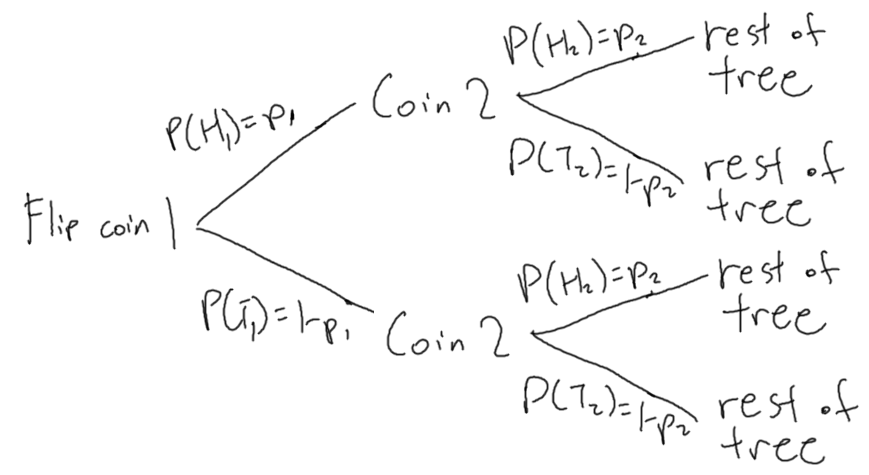
\includegraphics[width=8.5cm]{Diagram.png}
    \caption{A tree diagram that presents the situation of flipping all the coins.}
    \label{fig:my_label}
\end{figure}
Notice that each subtree starting from the same coin results in an identical scenario, meaning that everything is independent.

If we expand the generating function representing the first coin, we get 
\[F(x)=((1-p_1) + p_1 x)((1-p_2)+p_2x)\cdots ((1-p_n) + p_n x)\]\[=p_1 x((1-p_2) + p_2 x)((1-p_3)+p_3x)\cdots ((1-p_n) + p_n x) \]\[+ (1-p_1)((1-p_2) + p_2 x)((1-p_3)+p_3x)\cdots ((1-p_n) + p_n x).\]
The upper expression represents the upper portion of the tree, where we flip heads on coin 1. The $x$ indicates that we increase the total number of heads from flipping all the remaining coins by 1 and $p_1$ indicates the probability of flipping heads on coin 1.

The lower expression represents the lower portion of the tree, where we flip tails on coin 1. There is no exponent of $x$ because the number of heads does not increase from coin 1, but the value of $(1-p_1)$ represents the probability of flipping tails. Thus, the relationship between the tree and the generating function should be apparent. The expansion of the generating function one term at a time mimics the act of flipping and keeping track of which coins land heads and tails and with what probability.

In the full expansion of $F(x)$, the exponent of $x$ in for example the $k$ in $x^k$ represents the total number of heads flipped and the coefficient of $x^k$ represents the probability of flipping that many heads.

In essence, the act of expanding out equation \ref{coins} models every single possibility and its probability, since to extract a single term we must choose either the probability of heads or probability of tails for each coin and then add together the scenarios with the same number of total heads.

We can evaluate $F(-1)$ by using equation \ref{coins}. Remember that we assume that there is at least one fair coin and wish to prove that the probability of flipping an even number of heads is equal to the probability of flipping an odd number of heads. Assume for the sake of simplicity that the first coin is fair, or in other words $p_1=\frac{1}{2}$. Then, using equation \ref{coins},
\[F(-1)=((1-p_1) + p_1 (-1))((1-p_2)+p_2(-1))\cdots ((1-p_n) + p_n (-1)) \]\[= \left(\left(1-\frac{1}{2}\right)-\frac{1}{2}\right)((1-p_2)+p_2(-1))\cdots ((1-p_n) + p_n (-1))\]
\[= 0 \cdot ((1-p_2)+p_2(-1))\cdots ((1-p_n) + p_n (-1)) = 0.\] Clearly, it would not matter which coin was fair, since regardless, $F(-1)=0$.

We wish to find another meaning of $F(-1)=0$ which may be more useful, so we consider the expanded version of the generating function \[F(x)=\prod_{i=1}^n ((1-p_i) + p_i x)=a_0 + a_1 x + a_2 x^2 + \cdots + a_n x^n,\] where the coefficient $a_k$ is the probability of flipping exactly $k$ heads. For now, these variables $a_i, 0 \le i \le n$ are all placeholder variables since their values are unknown. However, consider the value of $F(-1)$. We first define $\alpha$ as the largest even number less than or equal to $n$ and $\beta$ as the largest odd number less than or equal to $n$. Then, Using the expression above, \[F(-1)=a_0 + a_1 (-1) + a_2 (-1)^2 + \cdots + a_n (-1)^n=a_0 - a_1 + a_2 - a_3 + \cdots + (-1)^n a^n\]
\begin{equation} \label{F(-1)}= (a_0 + a_2 + \cdots + a_{\alpha})-(a_1 + a_3 + \cdots + a_{\beta}).\end{equation} This expression is equal to the probability of flipping an even number of heads minus the probability of flipping an odd number of heads.

Then, by equation two, we know that \[F(-1)=(a_0 + a_2 + \cdots + a_{\alpha})-(a_1 + a_3 + \cdots + a_{\beta}) = 0\]\[\implies (a_0 + a_2 + \cdots + a_{\alpha})=(a_1 + a_3 + \cdots + a_{\beta}), \] which implies that the probability of flipping an even total number of heads is equal to the probability of flipping an odd total number of heads. \qed

Once again, this is not the only way to solve the "only if" direction. We can instead simply consider this argument. Consider isolating the fair coin and flipping all the other coins. The fair coin essentially "evens out" the probabilities. Suppose that there's a probability $p$ that after flipping all the coins except the fair coins that there are an even number of total heads, and that there's a probability $1-p$ that the total heads is odd. The fair coin has a $\frac{1}{2}$ probability of converting the probability $p$ of an even total to an odd total, and also has a $\frac{1}{2}$ probability of leaving it as is. The same thing applies for the scenario where all the other coins are tails. When the probabilities are added up for heads and tails, we find that it is $\frac{1}{2}$ for both, as desired.

However, the appeal of the usage of generating functions is that it allows for a greater understanding of the problem, which will be shown with the proof of the "if" direction.

\paragraph{The "if" direction}
In this section, we assume that there is an equal probability of flipping an even total number of heads as the probability of flipping an odd total number of heads.

Our goal is to roughly retrace the steps of our "only if" direction.

We define the same probabilities $p_i$ and $\alpha$ and $\beta$ as in the "only if" proof and use the same generating function \[F(x)=\prod_{i=1}^n ((1-p_i) + p_i x)=a_0 + a_1 x + a_2 x^2 + \cdots + a_n x^n.\]

Our assumption of the equal probabilities tells us that \[(a_0 + a_2 + \cdots + a_{\alpha})=(a_1 + a_3 + \cdots + a_{\beta})\]\[ \implies (a_0 + a_2 + \cdots + a_{\alpha})-(a_1 + a_3 + \cdots + a_{\beta}) = 0\]\[\implies a_0 (-1)^0 + a_1 (-1)^1 + \cdots + a_n (-1)^n = 0\]\[\implies F(-1)=0.\] \begin{sloppypar}Due to the factor theorem, since $F(-1)=0$ the polynomial $F(x)$ has a factor ${(x+1)}$. Then, for some $p_i, 0 \le i \le n$, we must have ${c((1-p_i) + p_i x)=x+1}$ for some constant $c$ for all $x$. By expanding and comparing coefficients, we have
${cp_i = 1, c-cp_i = c-1=1 \implies c=2 \implies p_i = \frac{1}{2}}$. Then, at least one of the coins must have an equal probability of flipping heads or tails, or in other words it is fair. \qed\end{sloppypar}

Once again, this is not the only way to complete the proof. This can also be done with a combination of proof by contradiction and proof by induction. However, the proof of these directions is relatively short when using generating functions compared to the proof by induction and contradiction, which demonstrates how these generating functions allow for insights about the problem as a whole to be easily made.
\section{Conclusion}
In this investigation, generating functions were used to prove identities and solve a counting problem.

In the proofs of the identities, the use of generating functions allowed for a much broader understanding of the identities, despite potentially requiring a longer proof. This may be because generating functions require broadness and generalization in order to be useful. However, this broadness allows for an understanding of these identities in relation to other similar identities.

In both the proof of Vandermonde's identity and the coin problem, generating functions provide a convenient way to model the situation abstractly. This abstraction allows for other tools to be used, such as multiplication of generating functions and the factor theorem. Furthermore, tools such as calculus were also used in conjunction with generating functions, which demonstrates how generating functions are a powerful and useful tool that only adds to the possibility of mathematics.

\section{Works Cited}
\begin{sloppypar}
Goemans, Michel. “What Is a Generating Function? - Massachusetts Institute of Technology.” \textit{MIT Mathematics}, 2015, \url{https://math.mit.edu/~goemans/18310S15/generating-function-notes.pdf}. 

Lerma, Miguel A. “PUTNAM TRAINING GENERATING FUNCTIONS.” \textit{Exercises - Math.northwestern.edu}, 2022, \url{https://math.northwestern.edu/putnam/training-genfunc.pdf}. 

Wilf, Herbert S. \textit{Generatingfunctionology}. Academic Press, 1994.

Zhao, Yufei. “Lecture 10 : A Contest of Contests - Yufei Zhao.” \textit{Yufei Zhao}, 2007, \url{https://yufeizhao.com/olympiad/comb3.pdf}. 


\end{sloppypar}
\end{document}
